\documentclass[12pt]{amsart}
%%%%%%%%%%%%%%%%%%%%%%%%%%%%%%%%%%%%%%%%%%%%%%%%%%%%%%%%%%%%%%%%%%%%%%%%%%%%%%%%%%%%%%%%%%%%%%%%%%%%%%%%%%%%%%%%%%%%%%%%%%%%%%%%%%%%%%%%%%%%%%%%%%%%%%%%%%%%%%%%%%%%%%%%%%%%%%%%%%%%%%%%%%%%%%%%%%%%%%%%%%%%%%%%%%%%%%%%%%%%%%%%%%%%%%%%%%%%%%%%%%%%%%%%%%%%   
\usepackage{amssymb}
\usepackage{amsmath}  
\usepackage{amsfonts}
\usepackage{mathrsfs}  
\usepackage{graphicx}
\usepackage{color}   
\usepackage[onehalfspacing]{setspace}
\usepackage{ragged2e}  
\justifying     
\usepackage{caption} 
\usepackage{etex} 
\usepackage{longtable} 
\usepackage{graphicx} 
\usepackage{amsmath}
\usepackage{multirow}
\usepackage{setspace}
\usepackage{footmisc}
\usepackage{amssymb}
\usepackage{amsfonts}
\usepackage[font=bf, justification=centering]{caption}
\usepackage{geometry}
\usepackage{float}
\usepackage{verbatim}
\usepackage{array}
\usepackage{booktabs}
\usepackage{pdflscape}
%\usepackage{xy} 
\usepackage{rotating}
\usepackage[round,authoryear]{natbib}
\usepackage{appendix}
\usepackage{lscape}
\usepackage{subcaption}
\usepackage{graphicx}
\usepackage{amsfonts}
\usepackage{placeins}
\usepackage[utf8]{inputenc}
\usepackage{charter}
\usepackage[colorlinks=true,citecolor=blue,urlcolor=blue,pdfpagemode=UseNone,pdfstartview=FitH]{hyperref}
\usepackage{apptools}
%\usepackage{chngcntr}
\usepackage{multibib}
\usepackage{multirow}
\DeclareUnicodeCharacter{00A0}{'}
%\usepackage[capposition=top]{floatrow}
\newcites{main,supp}{References,References}
%\AtAppendix{\counterwithin{lemma}{section}}
\makeatletter
\def\section{\@startsection{section}{1}
	\z@{1.0\linespacing\@plus\linespacing}{.5\linespacing}{\Large}}

\def\subsection{\@startsection{subsection}{2}
	\z@{.8\linespacing\@plus.7\linespacing}{.7\linespacing}{\large}}

\def\subsubsection{\@startsection{subsubsection}{3}
	\z@{.5\linespacing\@plus.7\linespacing}{-.5em}{\normalfont\bfseries}}
\makeatother                   

\setcounter{MaxMatrixCols}{10}
%TCIDATA{OutputFilter=LATEX.DLL}
%TCIDATA{Version=5.50.0.2953}
%TCIDATA{Codepage=936}
%TCIDATA{<META NAME="SaveForMode" CONTENT="1">}
%TCIDATA{BibliographyScheme=Manual}
%TCIDATA{LastRevised=Friday, May 08, 2015 15:13:41}
%TCIDATA{<META NAME="GraphicsSave" CONTENT="32">}
%TCIDATA{Language=American English}

\numberwithin{equation}{section}

\newtheorem{theorem}{Theorem}[section]
\newtheorem{lemma}{Lemma}[section]
\newtheorem{corollary}{Corollary}[section]
\theoremstyle{definition}
\newtheorem{definition}{Definition}[section]

\theoremstyle{definition}
\newtheorem{assumption}{Assumption}[section]

\theoremstyle{definition}
\newtheorem{example}{Example}[section]

\setlength{\textwidth}{6.5in}
\setlength{\textheight}{9in}
\setlength{\topmargin}{-0.1in}
\setlength{\oddsidemargin}{0in}
\setlength{\evensidemargin}{0in}
\vfuzz4pt
\hfuzz4pt
  

\title{}
\begin{document}
	\vspace*{3ex minus 1ex}
	\begin{center}
		\Large \textsc{Love your Incubment but Hate his Party: \\ The Asymmetric Effect of Reelection on Partisan and Personal Incumbency Returns}
		%\bigskip  
	\end{center}
	
	
\date{April 23, 2021} 
\vspace*{3ex minus 1ex}
	\begin{center}
		Rafael Ch\\
		
		\textit{New York University}\\
		
	\end{center}
	 
	\thanks{%I thank Pablo Querubin, Cyrus Samii, Hye Young You, Neal Beck, Jacob Shapiro, Juan F. Vargas, Nicholas Haas, Reed Lei, Lucia Motolinia and participants at the Summer Cohort Seminar, Graduate Political Economy Seminar, and Comparative Politics Seminar at NYU, APSA 2020, SPSA 2021, and MPSA 2021 panelists, as well as the members of the Methods and Data Seminar at the University of Wisconsin-Madison for their amazing comments and suggestions. All mistakes are my own.
	\\
	 \\ \textbf{Ch:} Wilf Family Department of Politics, New York University. \\ Email: \url{rafael.ch@nyu.edu}
	 \\ Website: \url{https://wp.nyu.edu/rafaelch/}}
		  
	\begin{abstract}    
	
A large literature has studied the electoral returns to incumbency. However, the incumbency return in the next election -whether positive or negative- masks an understudied dynamic between parties and their members: they can both be hated, both loved or asymmetrically liked by the constituency. This paper opens up the black box of incumbency by studying the effect of reelection on personal and partisan incumbency returns. To do so, I exploit the staggered implementation of an electoral reform that introduced reelection for local executives from 2014 to 2022 in Mexico, a party-centered system. I find that a seemingly null result hides an incumbency asymmetry: when citizens are able to reelect the incumbent a personal incumbency advantage follows, with parties suffering from an incumbency disadvantage. Contrary to past studies, a difference-in-discontinuity in close elections allows me to overcome methodological downfalls, primarily the difference in experience and ability between term limited and non non-term limited incumbents, as well as rule out the differential trends on electoral returns that localities may have. Results suggest the personal advantage to be driving positive incumbency returns when reelection exists even in party-centered systems. 
	
    
	\medskip
	{\noindent \textsc{Key words: Reelection, Incumbency Advantage, Incumbency Disadvantage, Resources, Politician Quality, Performance in Office.}}

		%{\noindent \textsc{JEL Classification: %D72, D78, H57, O17.}}
	\end{abstract}
	
	\maketitle
	\pagebreak
%\section*{Abstracts}
   

\clearpage
\section{Main Results}

  
 \begin{figure}[H]   
\centering    
 \caption{Effect of Term Limit Reform on Partisan and Personal Incumbency Advantage \\ -difference-in-discontinuity of close elections design-}
 \label{fig:personal_vs_partisan}
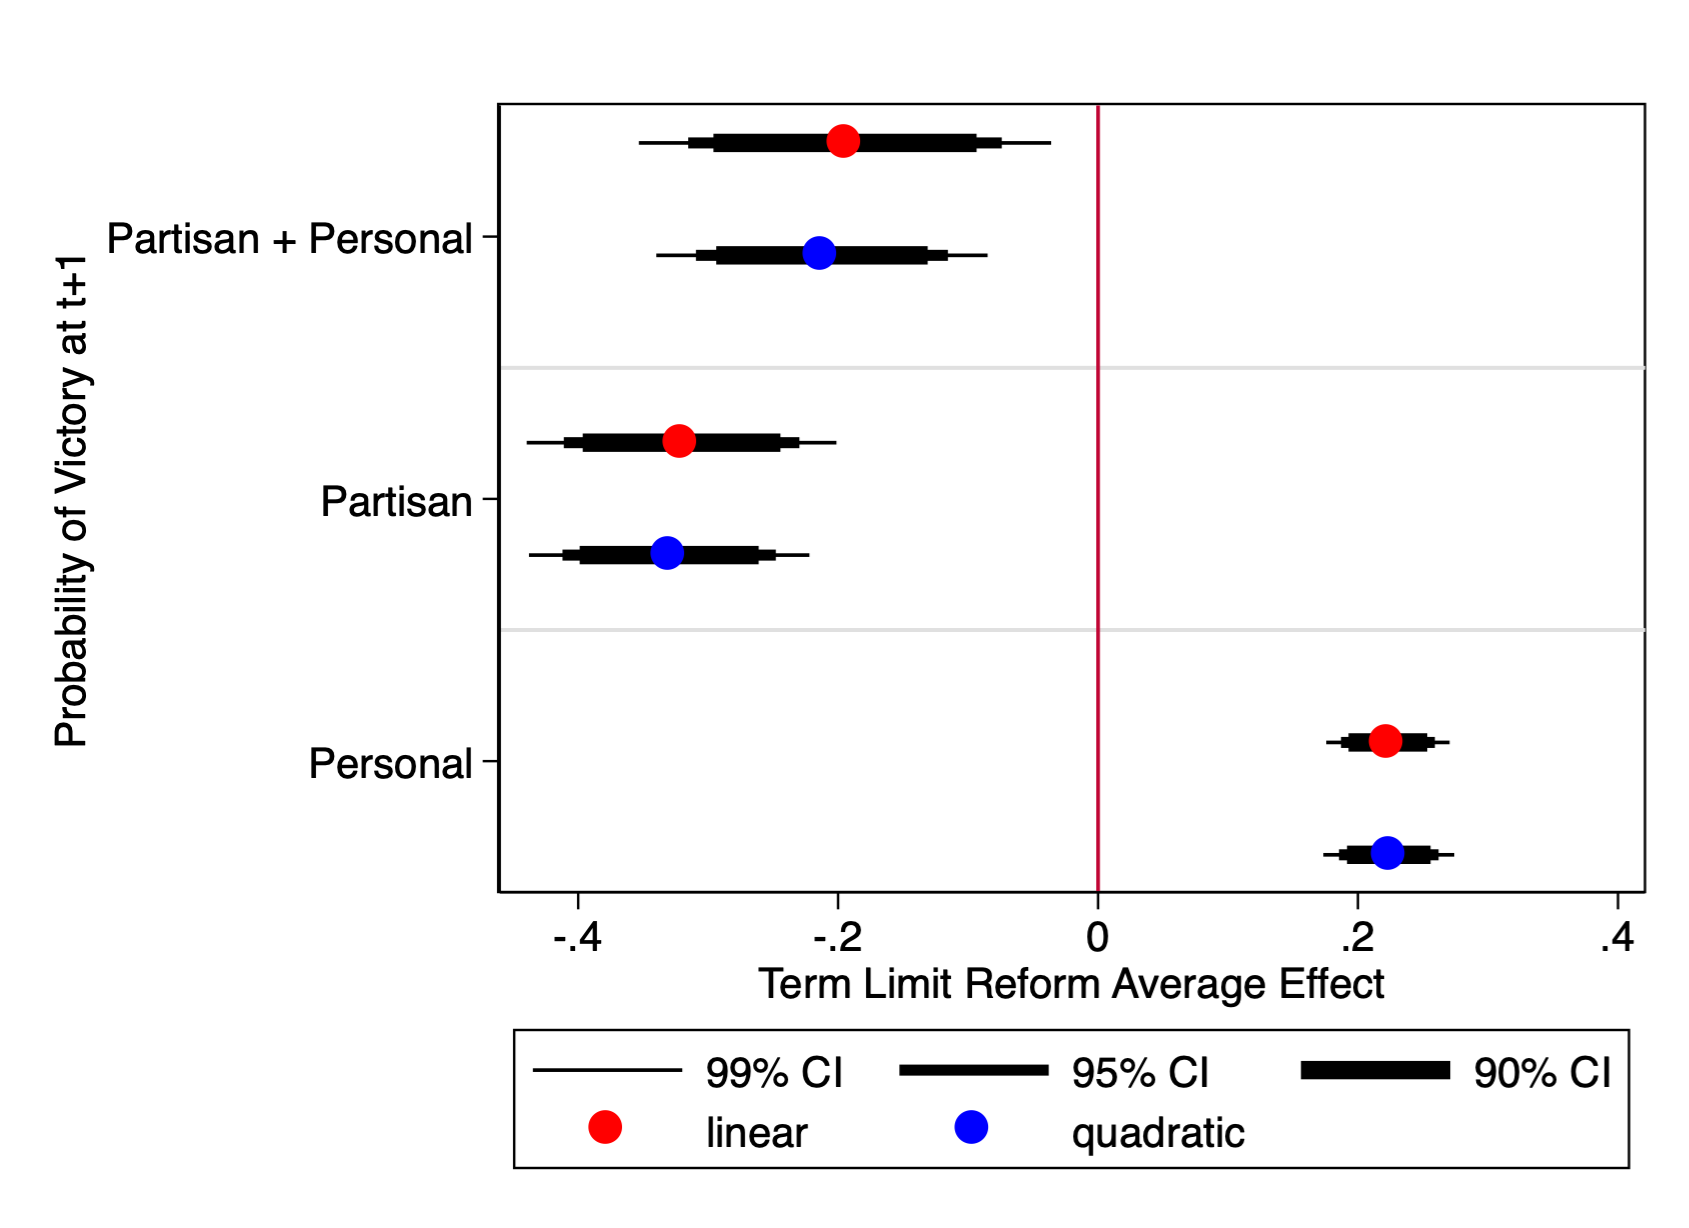
\includegraphics[width=0.9\textwidth]{../Figures/partisan_personal_inc_advantage.png}
       \captionsetup{justification=centering}
       
 \textbf{Note:} Figure \ref{fig:personal_vs_partisan} shows the average treatment effect of the Term Limit Reform on the probability of winning in the following election using a difference in discontinuity of close elections design. This average effect was estimated using the IW estimators following \citet{abraham_sun_2020} for each lead and lag relative to the first year a municipality implemented reelection. Optimal bandwidths following \citet{calonicoetal_2014} are used. This analysis identifies the party that wins at $t-1$ and studies the effect of this party barely winning (or losing) at $t$ on outcomes at election $t+1$ following \citet{klasnja_titiunik_2017}. I follow \citet{fowler_hall_2014} to decompose the incumbency advantage into the partisan and personal component. Red and blue points show that parallel trends hold, while hollow ones imply pretrends. 
\end{figure}  

   
\clearpage
\section{Robustness}


\begin{table}[htbp]\def\sym#1{\ifmmode^{#1}\else\(^{#1}\)\fi}
\centering
\caption{Event-in-Discontinuity in close elections model: Effect of 2014 Term Limit Reform on Incumbency Advantage}
\label{tab:incumbency_wpolynomials}
\scalebox{0.8}{
\begin{tabular}{lcc}
\hline \hline
\\ \multicolumn{3}{l}{Dependent variable:}\\
& \multicolumn{1}{c}{Incumbent at t-1 won at t+1}  & \multicolumn{1}{c}{Incumbent at t won at t+1} \\
& \multicolumn{1}{c}{(indicator)}  & \multicolumn{1}{c}{(indicator)} \\
& \multicolumn{1}{c}{(1)} & \multicolumn{1}{c}{(2)}  \\
\cmidrule(lrr){2-2}  \cmidrule(lrr){3-3} \\
\addlinespace
& \multicolumn{2}{c}{linear polynomial} \\
\cmidrule(lrr){2-3} \\
4 Elections prior &       $ -0.0006^{} $ &       $ 0.0578^{*} $  \\
& ($ 0.0681 $ ) & ($ 0.0320 $ ) \\
3 Elections prior &       $ 0.0747^{} $ &        $ -0.1118^{***} $ \\
& ($ 0.1660 $ ) & ($ 0.0343 $ ) \\
2 Elections prior &          $ 0.1262^{} $ &       $ 0.0773^{} $ \\
& ($ 0.0965 $ ) & ($ 0.1420 $ ) \\
Election after Reform &         $ -0.0025^{} $ &        $ 0.1355^{***} $ \\
& ($     . $ ) & ($     . $ ) \\
Observations          &              2,002     &              3,084 \\
R-squared        &          0.5605   &          0.5887 \\
\\
& \multicolumn{2}{c}{quadratic polynomial} \\
\cmidrule(lrr){2-3} \\
4 Elections prior &       $ -0.1093^{***} $ &       $ 0.0657^{} $  \\
& ($ 0.0144 $ ) & ($ 0.0433 $ ) \\
3 Elections prior &       $ 0.3221^{***} $ &        $ -0.2892^{***} $ \\
& ($ 0.0608 $ ) & ($ 0.0557 $ ) \\
2 Elections prior &          $ 0.0467^{} $ &       $ 0.0358^{} $ \\
& ($ 0.0801 $ ) & ($ 0.1267 $ ) \\
Election after Reform &         $ -0.1600^{***} $ &        $ 0.1111^{***} $ \\
& ($     . $ ) & ($     . $ ) \\
Observations          &              2,766     &              4,038 \\
R-squared        &          0.5478   &          0.4066 \\
\\
Mun. FEs        &     \checkmark         &  \checkmark   \\
Year. FEs     &     \checkmark         &  \checkmark  \\
Controls$^a$  &    \checkmark     &       \checkmark \\
Cohort weighted  &         \checkmark &         \checkmark \\
\hline \hline
\multicolumn{3}{p{0.9\textwidth}}{\footnotesize{Notes: Coefficients show IW estimators following \citet{abraham_sun_2020}. Two relative time periods (lag 6 and 1) are removed to avoid collinearity problems noted by \citet{abraham_sun_2020} or because they are collinear or inexistent, like lag time period 2. Standard errors in parentheses are clustered at the state level for estimates in saturaded model. Significance-level: $^{***}$ 1\%; $^{**}$ 5\%; and $^*$ 10\%, that refer to two-sided t-test with the null hypothesis equal to 0 for each relative time period. $^a$ State-level controls include governor winning margin in last pre-treatment election and an indicator of whether the governor's party is the same as the federal incumbent party. Logged homicides per capita at the municipality level are also included as controls.}} \\
\end{tabular}
}
\end{table}
   
   
 \begin{figure}[H]   
\centering
 \caption{Effect of Term Limit Reform on Partisan and Personal Incumbency Advantage \\ -difference-in-discontinuity of close elections-}
 \label{fig:parallel_trend}
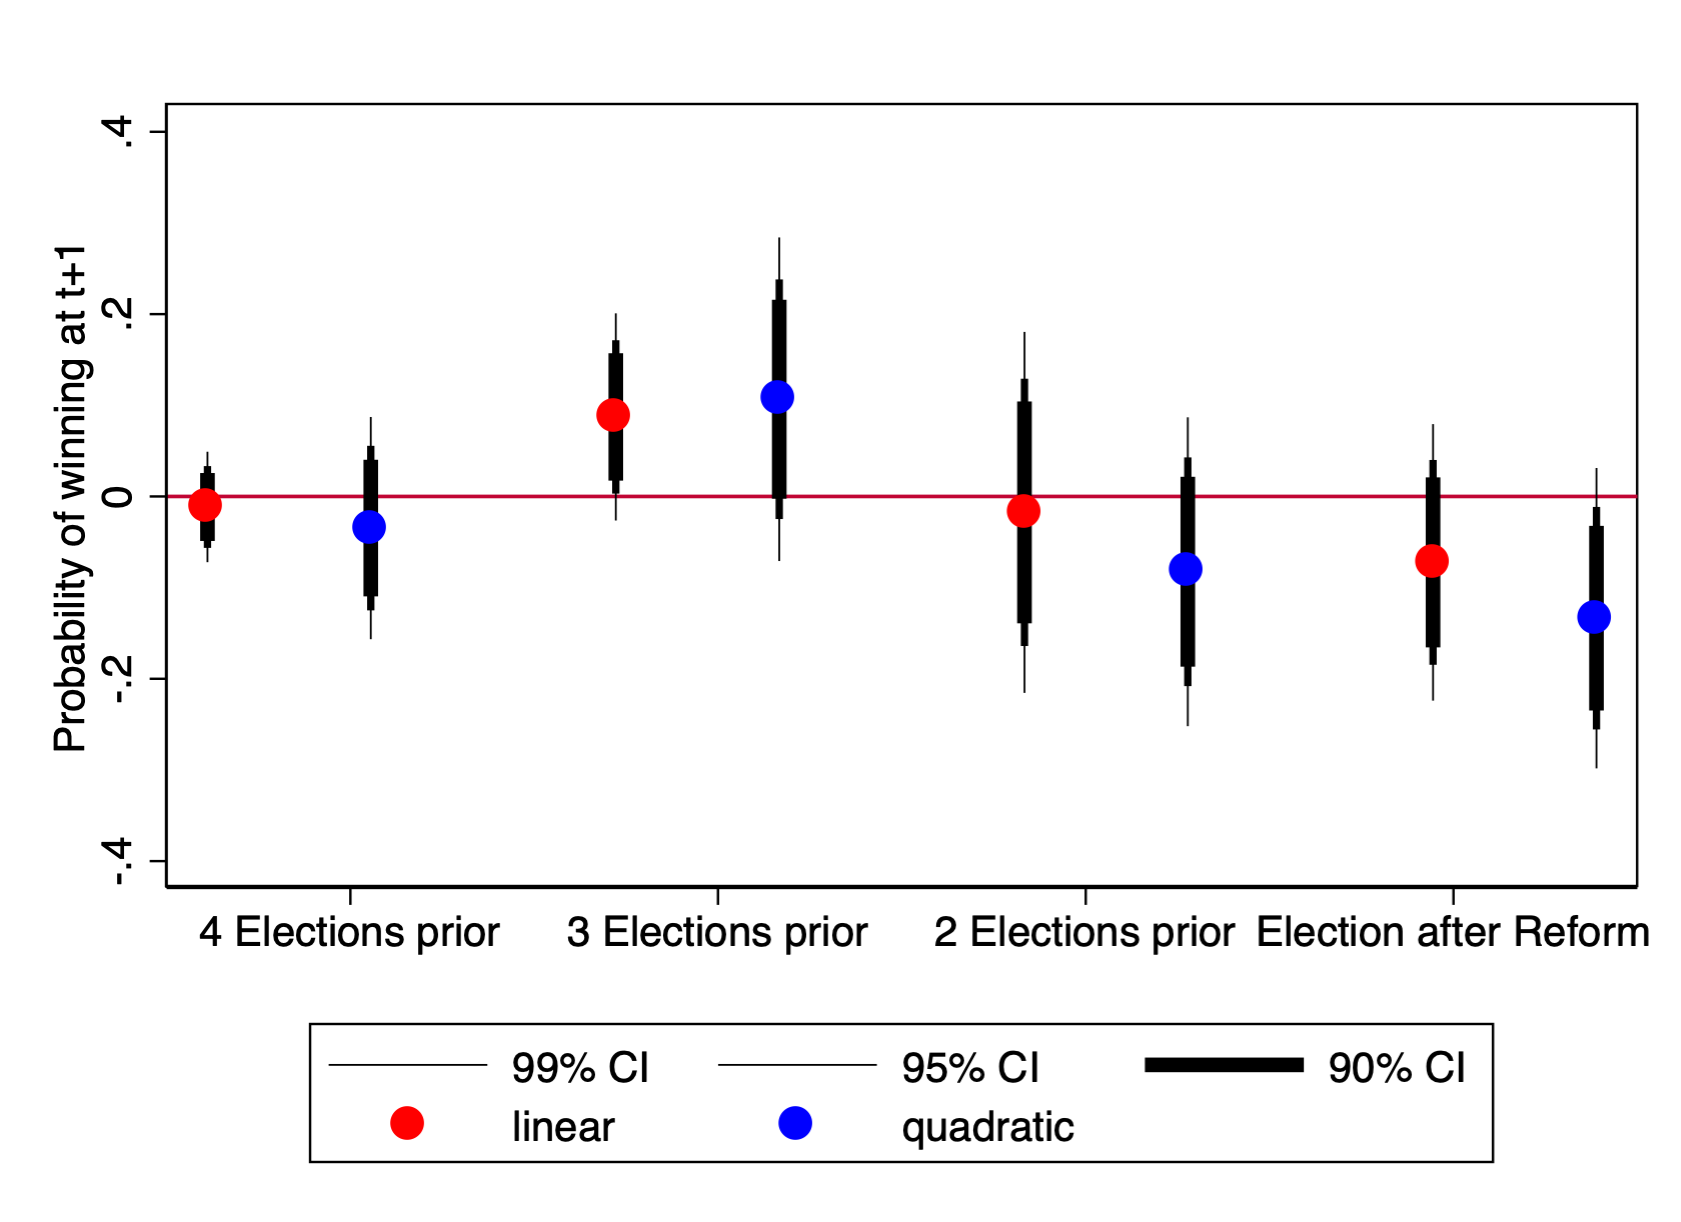
\includegraphics[width=0.9\textwidth]{../Figures/parallel_trends_incumbency.png}
       \captionsetup{justification=centering}
         
 \textbf{Note:} Figure \ref{fig:parallel_trend} shows the average treatment effect of the Term Limit Reform on the probability of winning in the following election using a difference in discontinuity of close elections design. This average effect was estimated using the IW estimators following \citet{abraham_sun_2020} for each lead and lag relative to the first year a municipality implemented reelection. Optimal bandwidths following \citet{calonicoetal_2014} are used. This analysis identifies the party that wins at $t-1$ and studies the effect of this party barely winning (or losing) at $t$ on outcomes at election $t+1$ following \citet{klasnja_titiunik_2017}.  
 
\end{figure}  


 \begin{figure}[H]   
\centering
 \caption{McCrary Test}
 \label{fig:mcrary}
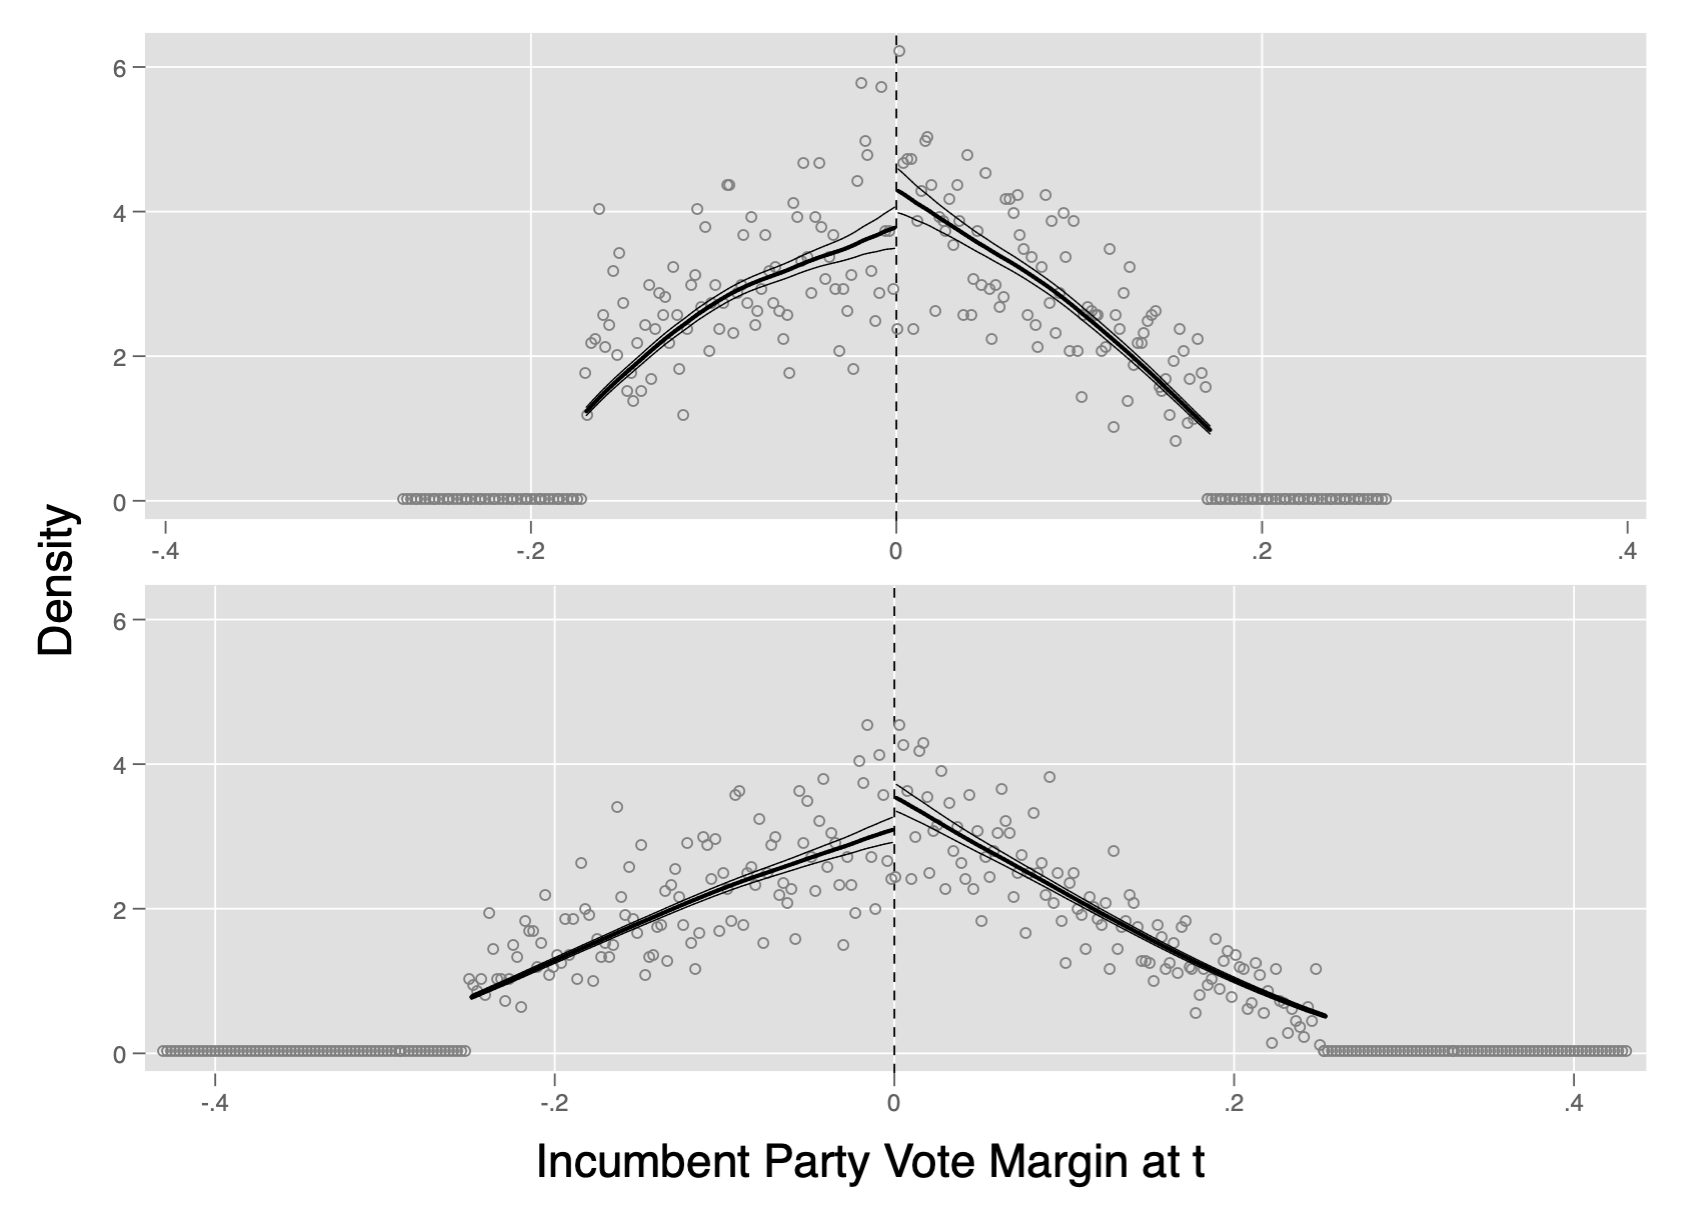
\includegraphics[width=0.9\textwidth]{../Figures/conditional_mccrary_test_pol1_final.png}
       \captionsetup{justification=centering}
         
 \textbf{Note:} 95\% confidence intervals reported. With 90\% levels confidence intervals overlap..  
 
\end{figure} 

 \begin{figure}[H]   
\centering
 \caption{No discontinuous jump of covariates}
 \label{fig:parallel_trend}
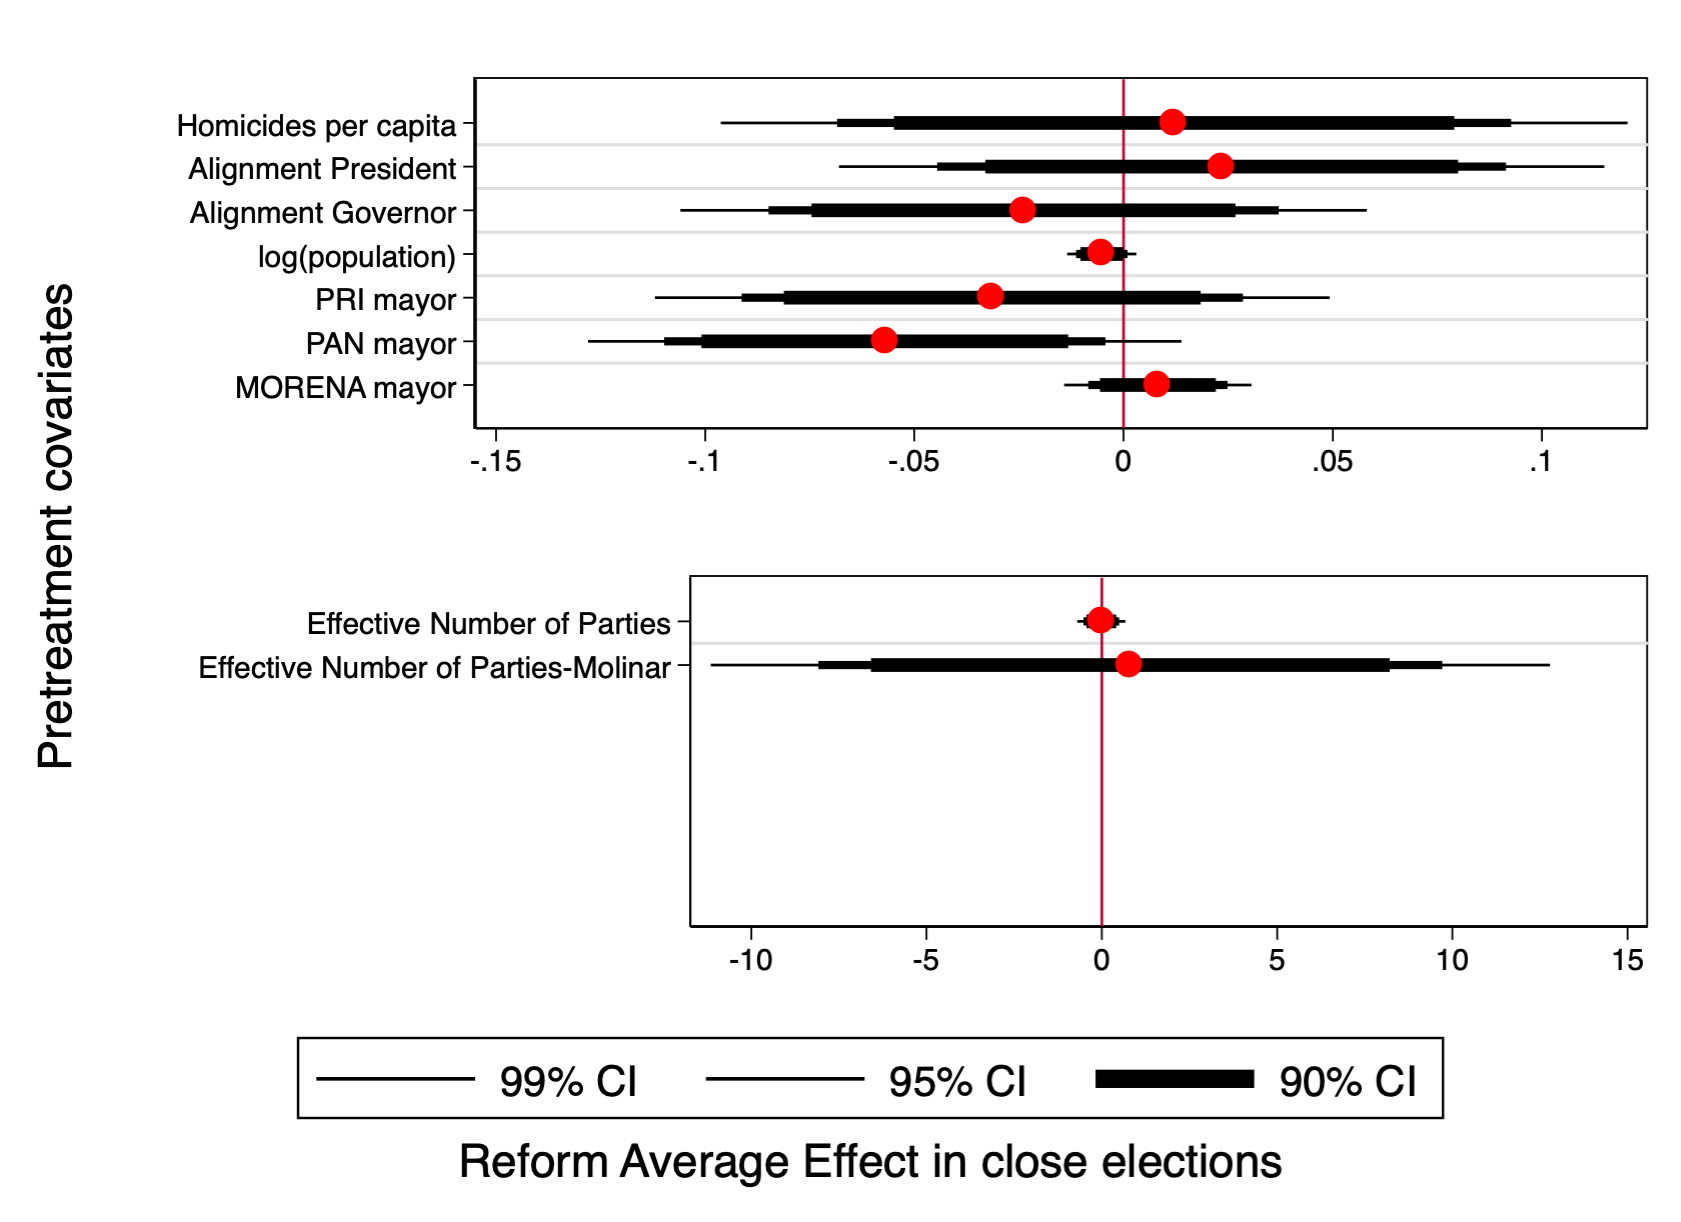
\includegraphics[width=0.9\textwidth]{../Figures/nojump.png}
       \captionsetup{justification=centering}
    
 %\textbf{Note:}.  
   
\end{figure} 


 \begin{figure}[H]   
\centering
 \caption{Testing Different Bandwidths}
 \label{fig:parallel_trend}
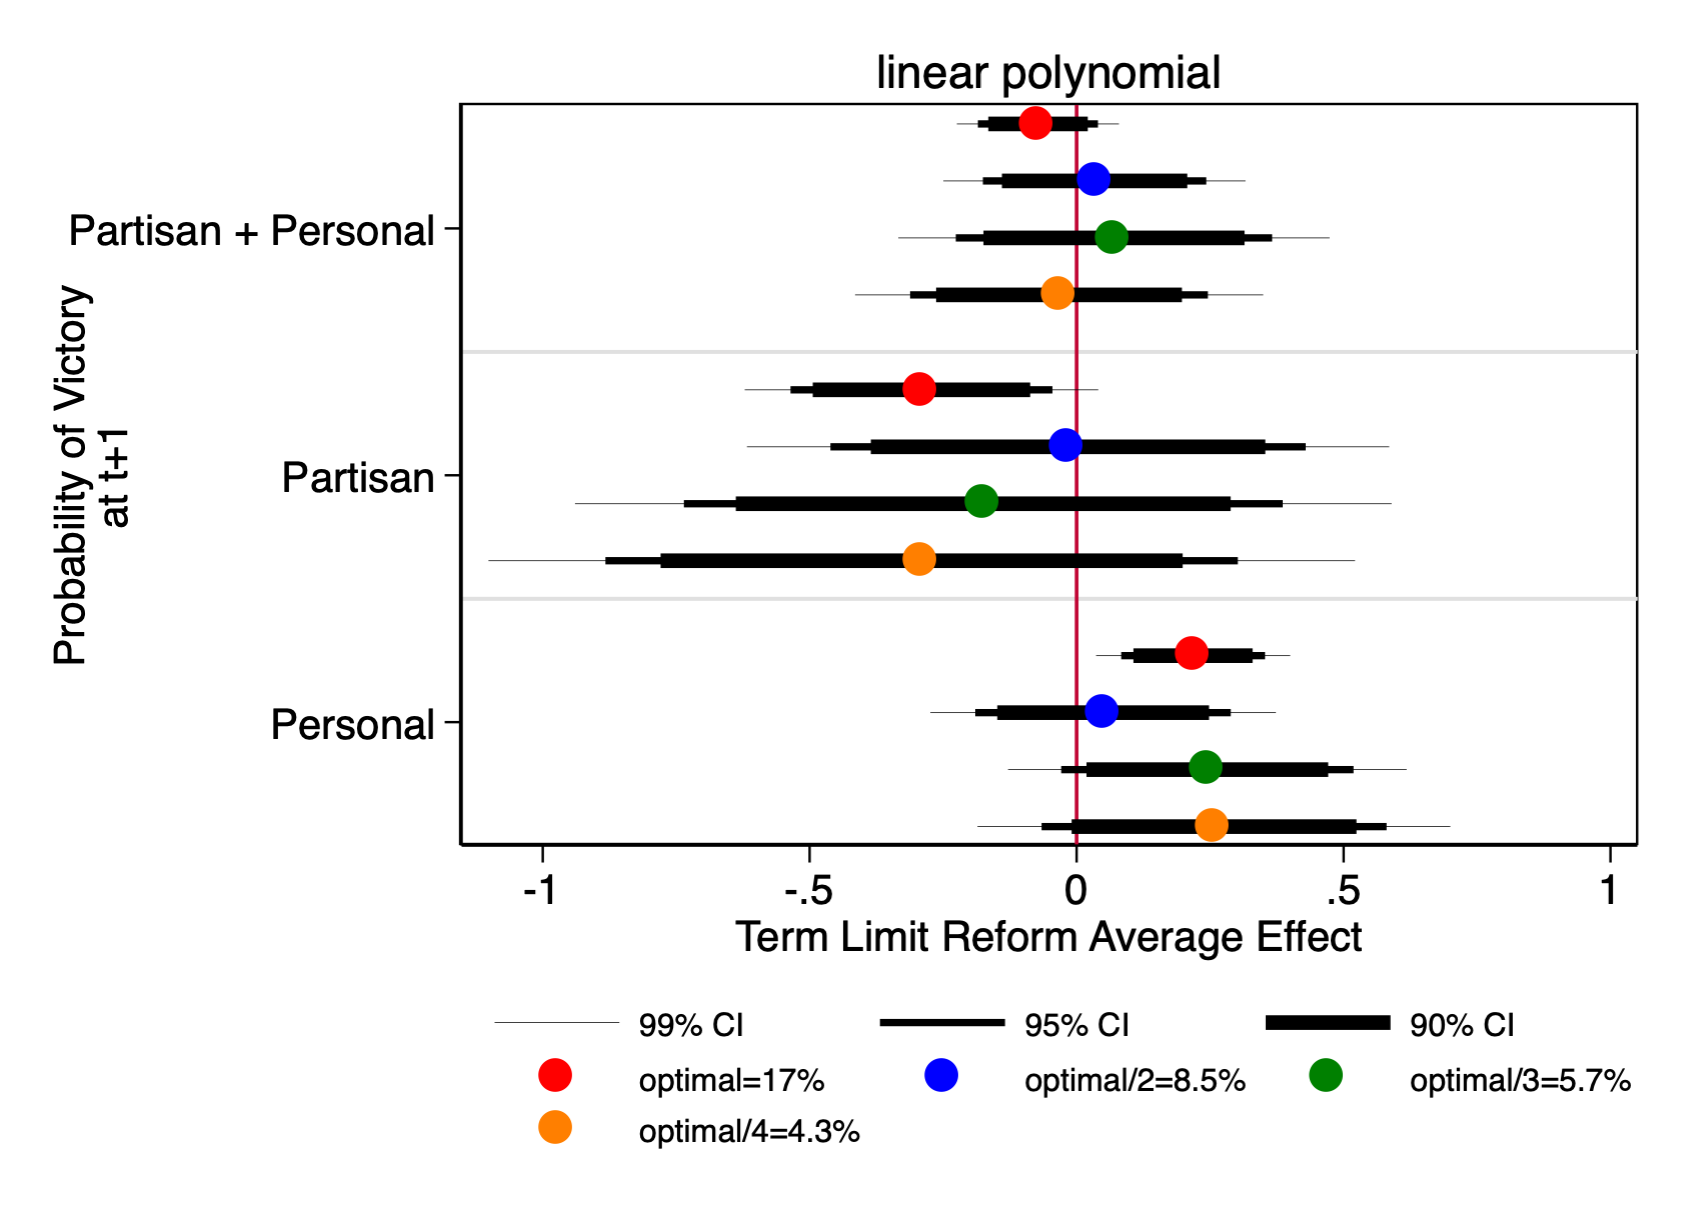
\includegraphics[width=0.9\textwidth]{../Figures/many_bandwidths_linear.png}
       \captionsetup{justification=centering}
 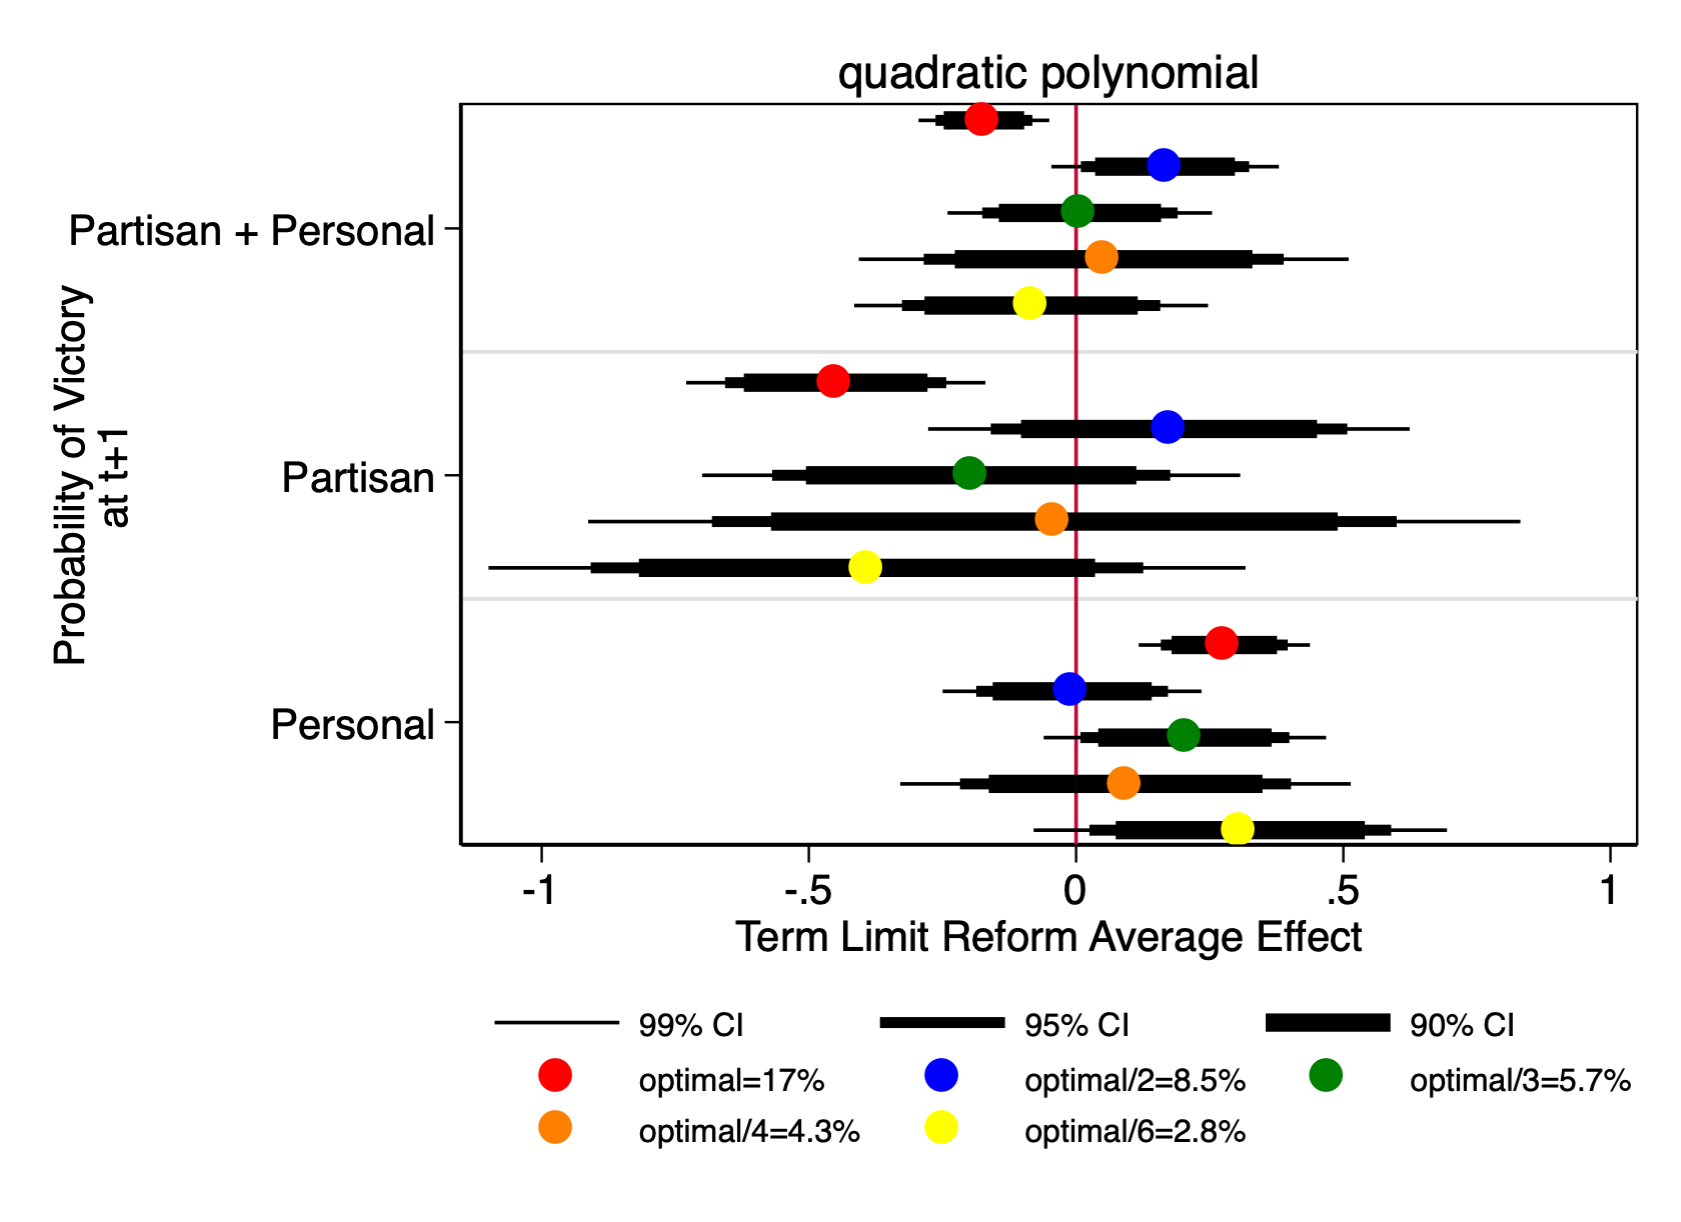
\includegraphics[width=0.9\textwidth]{../Figures/many_bandwidths_quadratic.png}

 %\textbf{Note:}.  
   
\end{figure} 



\clearpage

\section{Mechanisms}

\clearpage

 
\clearpage
\section{New Appendix}

\subsection{Main Results}

 
\subsection{Robustness}

\clearpage

\subsection{Mechanisms}
    
 \clearpage   
            
%APPENDIX -----------------------------------------------

%%%%%%%%%%%%
\bibliographystyle{aer} 
\bibliography{References}    

\clearpage
%APPENDIX -----------------------------------------------
\begin{appendix}
\renewcommand{\thetable}{A-\arabic{table}}
\setcounter{table}{0}
 
\renewcommand{\thefigure}{B-\arabic{figure}}
\setcounter{figure}{0}

   
%%%%%%%%%%%%%%%%%%%%%%%%%%%%%%%%% 

  
\end{document}
